
\section{Experimental results}

\subsection{Data}

\subsubsection{Training data}

\subsubsection{Test data}\label{sec:test_data}
\cite{mikolov3} propose evaluating the regularities of the learned embedding space with a test set of analogy questions. The questions are of the form "{\it a} is to {\it b} as {\it c} is to \_\_ ". The test set contains 14 different types of analogies (see Table \ref{table:analogical}) relating to semantic concepts and grammatical relations. 

\begin{table}[h]
\small
	\caption{Analogical reasoning test set}
	\label{table:analogical}
	\centering
    \begin{tabular}{| c |  c | c |}
    \hline
    {\bf Relation} & {\bf \# Questions} & {\bf Example} \\
    \hline
     capital-common-countries & 506 & Athens : Greece \\
     & & Bangkok : Thailand\\
     \hline
    capital-world &   4524  & Abuja : Nigeria \\
    & & Accra : Ghana\\
    \hline
    currency & 866 & Algeria : dinar\\
    & & Japan : yen\\
   \hline
   city-in-state & 2467 & Chicago : Illinois \\
   & & Houston Texas\\
   \hline
    family &  506 & brother : sister \\
    & & mother : father\\
    \hline
    adjective-to-adverb & 992 & amazing : amazingly \\
    & & calm : calmly\\
    \hline
    opposite & 813 & acceptable : unacceptable \\
    & & aware : unaware\\
    \hline
    comparative & 1331 & bad : worse \\
    & & big : bigger\\
    \hline
    superlative & 1122 & bad : worst \\
    & & big : biggest\\
    \hline
    present-participle & 1056 & code : coding\\
    & & dance : dancing\\
    \hline
    nationality-adjective & 1599 & Albania : Albanian \\
    & & Argentina : Argentinean\\
    \hline
    past-tense & 1560 & dancing : danced \\
    & & decreasing : decreased\\
    \hline
    plural & 1332 & banana : bananas \\
    & & bird birds\\
    \hline
    plural-verbs &  & eat : eats \\
    & 870 & generate : generates\\
    \hline
    \end{tabular}
\end{table}


\subsection{Results}

\subsubsection{Measuring linguistic regularity via analogies}
We evaluate the performance of (a) pre-trained Google vectors, (b) our Skip-Gram model, (c) our CBOW model, on the analogical reasoning test set introduced in section \ref{sec:test_data}. Given three query words (e.g. {\it Paris, France, London}), the task is to return the answer that fits with the analogy (in this case, {\it England}). This problem can be solved in many ways, \cite{mikolov1} propose a simple solution that relies on the inherent regularities of the embedding space learned by the Skip-Gram and CBOW models. The method uses simple vector algebra in the embedding space to find the solution word given three query words. For example, suppose the analogical relation of interest is {\it A} is to {\it B} as {\it} C is to {\it D}. Given three query words, {\it A, B, C}, the predicted solution is computed as follows:
\begin{enumerate}
\item Compute the vector representations of each word, $\phi(A), \phi(B), \phi(C)$.
\item Let $v = \phi(B) - \phi(A) + \phi(C)$.
\item Do a nearest neighbors search, based on cosine distance, to find the $K$ closest word vectors to $v$. In other words, solve for the top $K$ solutions to 
	\begin{align} \max_u\frac{ v \cdot u}{\| u \| \| v \|}\ \end{align}
\end{enumerate}

The intuition behind this method is that the cosine distance between $\phi(A - B)$ and $\phi(C - D)$ is small when {\it A} and {\it B} are analogous to {\it C} and {\it D}. Figure \ref{fig:offsets} illustrates this intuition. 

\begin{figure}[h]
\centering
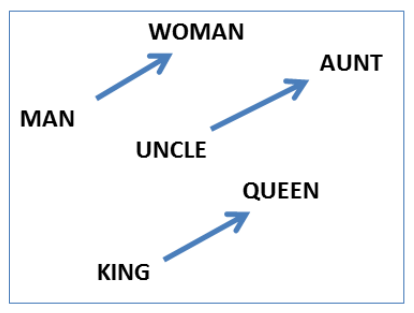
\includegraphics[width=.45\textwidth]{./images/king_queen.png}
\caption{Vector offsets for three analogous word pairs.}
\label{fig:offsets}
\end{figure}

Table \ref{tab:analogical_acc} shows the top-$k$ accuracy on the analogical reasoning dataset of the pre-trained Google vectors (GoogleVec) and the Skip-Gram and CBOW models that we trained. The Google vectors outperform both our versions for all $k$. This is to be expected since the Google vectors were trained on far more data than we have access to. 

Our CBOW model performs consistently worse than our Skip-Gram model. We hypothesize that this is a factor of the amount of training data we used to train our models. The CBOW model throws away a lot of information by ignoring the ordering of words. In the limit of infinite data, the bag-of-words assumption might not matter, however in a limited data setting we believe the CBOW model is hurt more than the Skip-Gram model due to the loss of information. 

Figure \ref{fig:top_k} plots the top-$k$ accuracy as a function of $k$ for the three models split up by analogy types. Figure \ref{fig:accuracy_per_question}  plots the top-5 accuracy of the three models for each of the analogy question types. A very interesting pattern emerges when we consider these results. We can break down the analogy questions into two type: (1) Analogies involving semantic relations between words such as capital-country, currency-country, and family relations (1) Grammatical analogies such as past/present tense. singular/plural terms, and present-participle relations. We notice that the Skip-Gram model performs better on analogical questions of type (1) whereas the CBOW model performs better on the questions of type (2). We hypothesis that this is a function of the number of examples of each kind of relation. The semantic analogies appear in very specific contexts. For example, the word {\it France} is unlikely to appear in general text but would rather appear in particular contexts. However, words in the grammatical relations are not specific to a particular context and would appear in a very wide variety of sentences. Thus, we hypothesize that the models have, in some sense, more information about grammatical relations than they do about specific semantic relations during training. Thus, since the CBOW model performs better when there is more data available, the CBOW model performs worse on semantic analogical relations than grammatical ones. 


\begin{table}[h]
	\caption{Top k Accuracy on Analogical Reasoning Test}
	\label{tab:analogical_acc}
	\centering
    \begin{tabular}{| c | c | c | c |}
    \hline
    \textbf{Top k} & \textbf{GoogleVec} & \textbf{CBOW} & \textbf{Skip-Gram}\\ \hline
    1 & 20.185\% & 3.029\% & 6.211\%  \\ \hline
    2 & 68.967\% & 24.764\%& 46.986\% \\ \hline
    3 & 78.346\% & 37.919\%& 59.179\% \\ \hline
    4 & 82.424\% & 43.921\%& 65.314\% \\ \hline
    5 & 84.716\% & 47.513\%& 68.967\% \\ \hline
    6 & 86.246\% & 50.332\%& 71.479\% \\ \hline
    7 & 87.285\% & 52.553\%& 73.362\% \\ \hline
    8 & 88.149\% & 54.308\%& 74.631\% \\ \hline
    9 & 88.835\% & 55.879\%& 75.716\% \\ \hline
    10 & 89.352\% & 57.142\%& 76.698\% \\ \hline
    \end{tabular}
\end{table}


\begin{figure}[h]
\centering
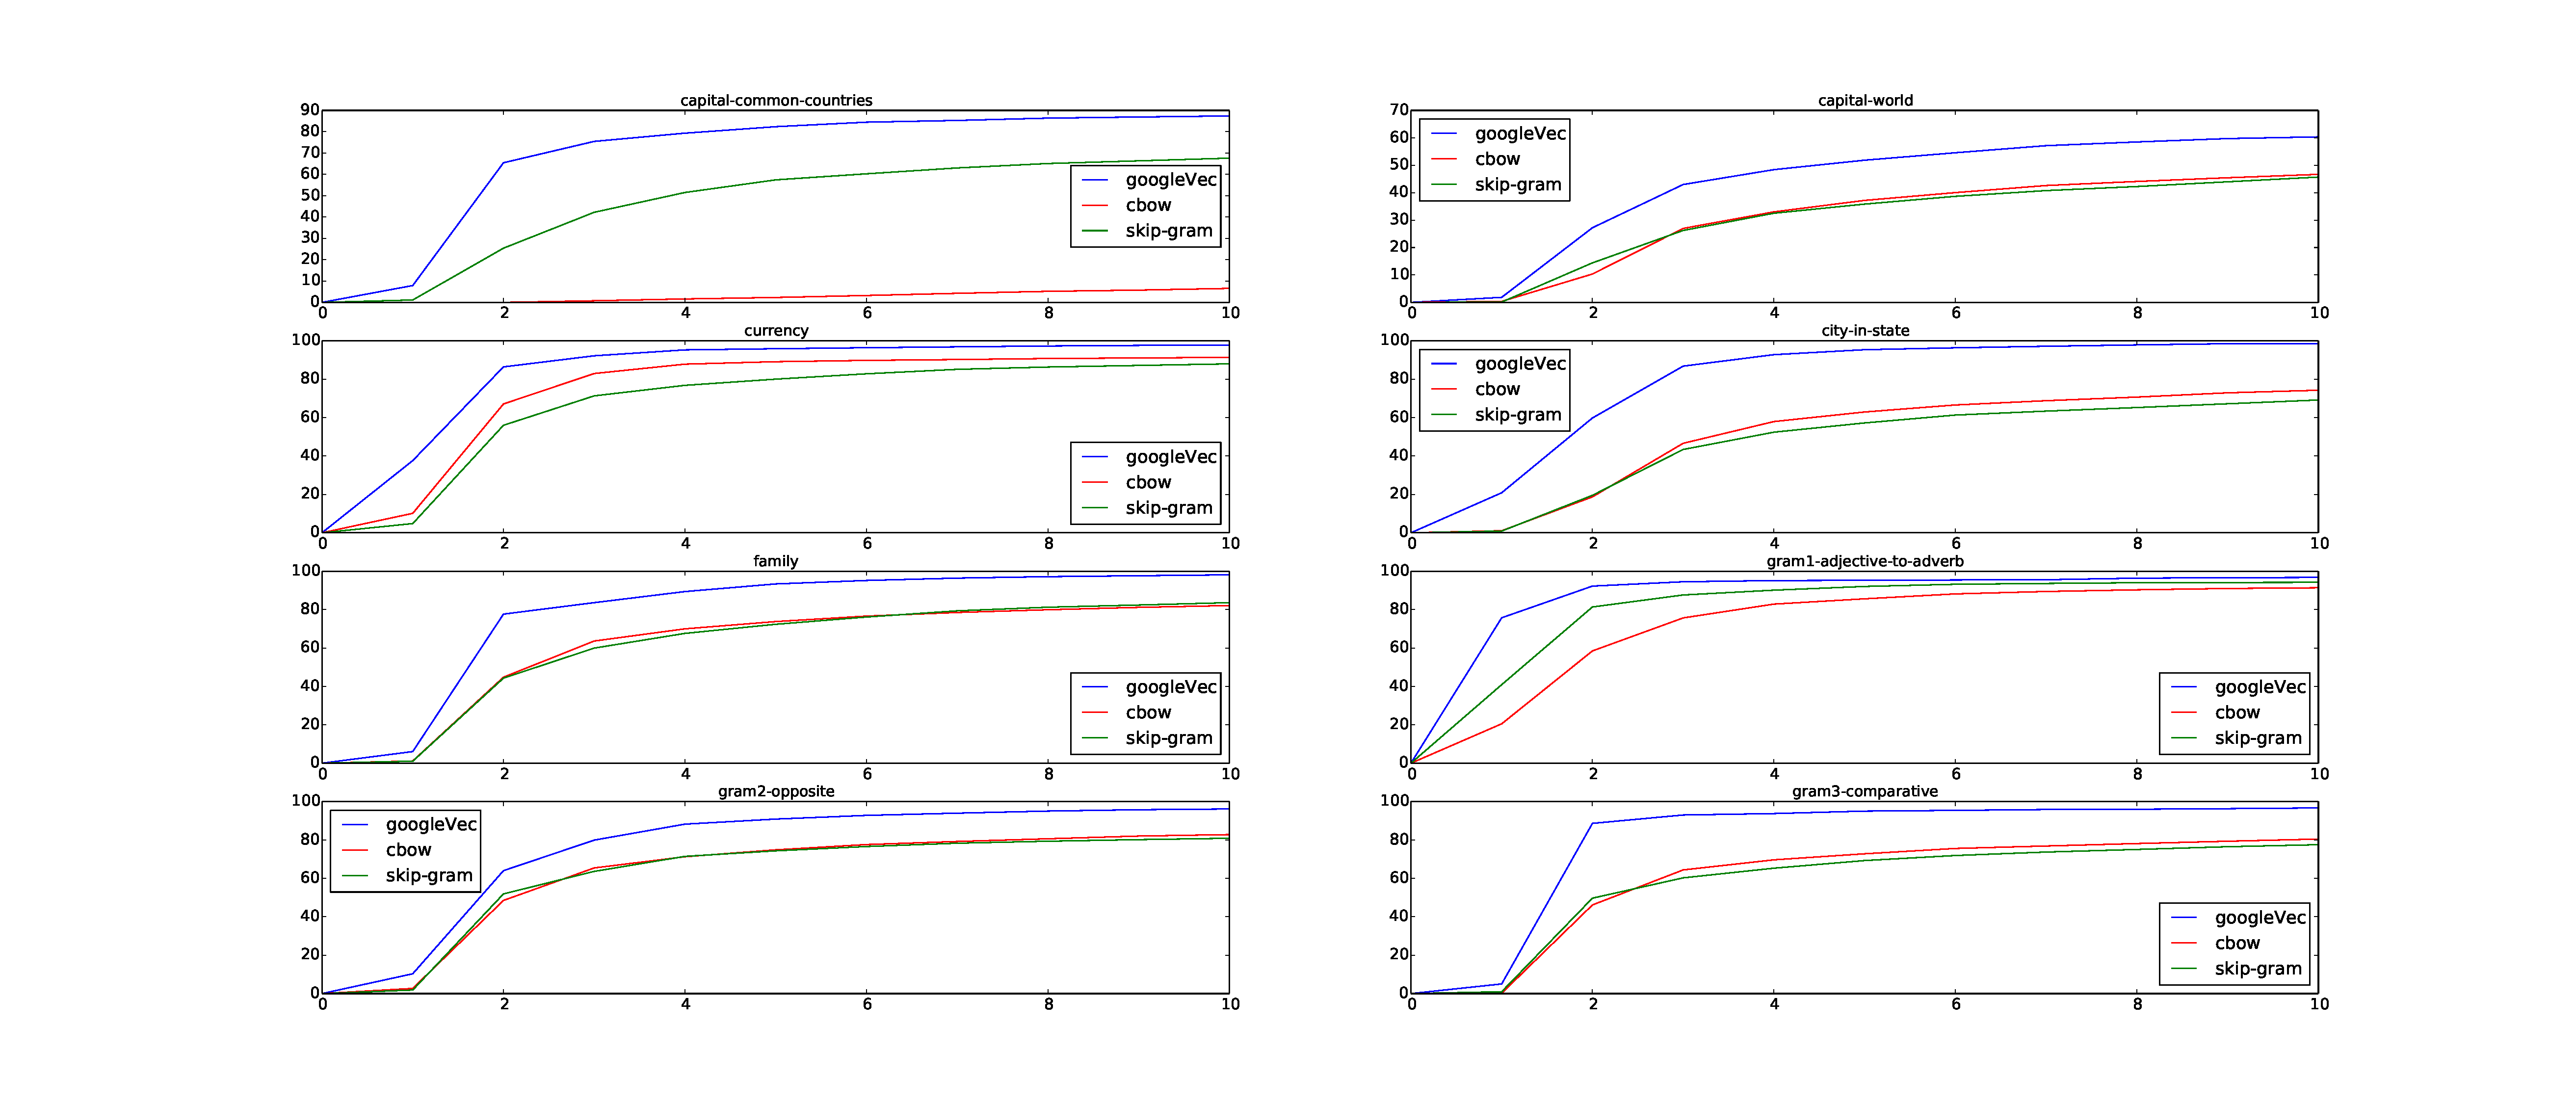
\includegraphics[width=\textwidth]{./images/top_k.pdf}
\caption{Top K accuracy for increasing K.}
\label{fig:top_k}
\end{figure}

\begin{figure}[h]
\centering
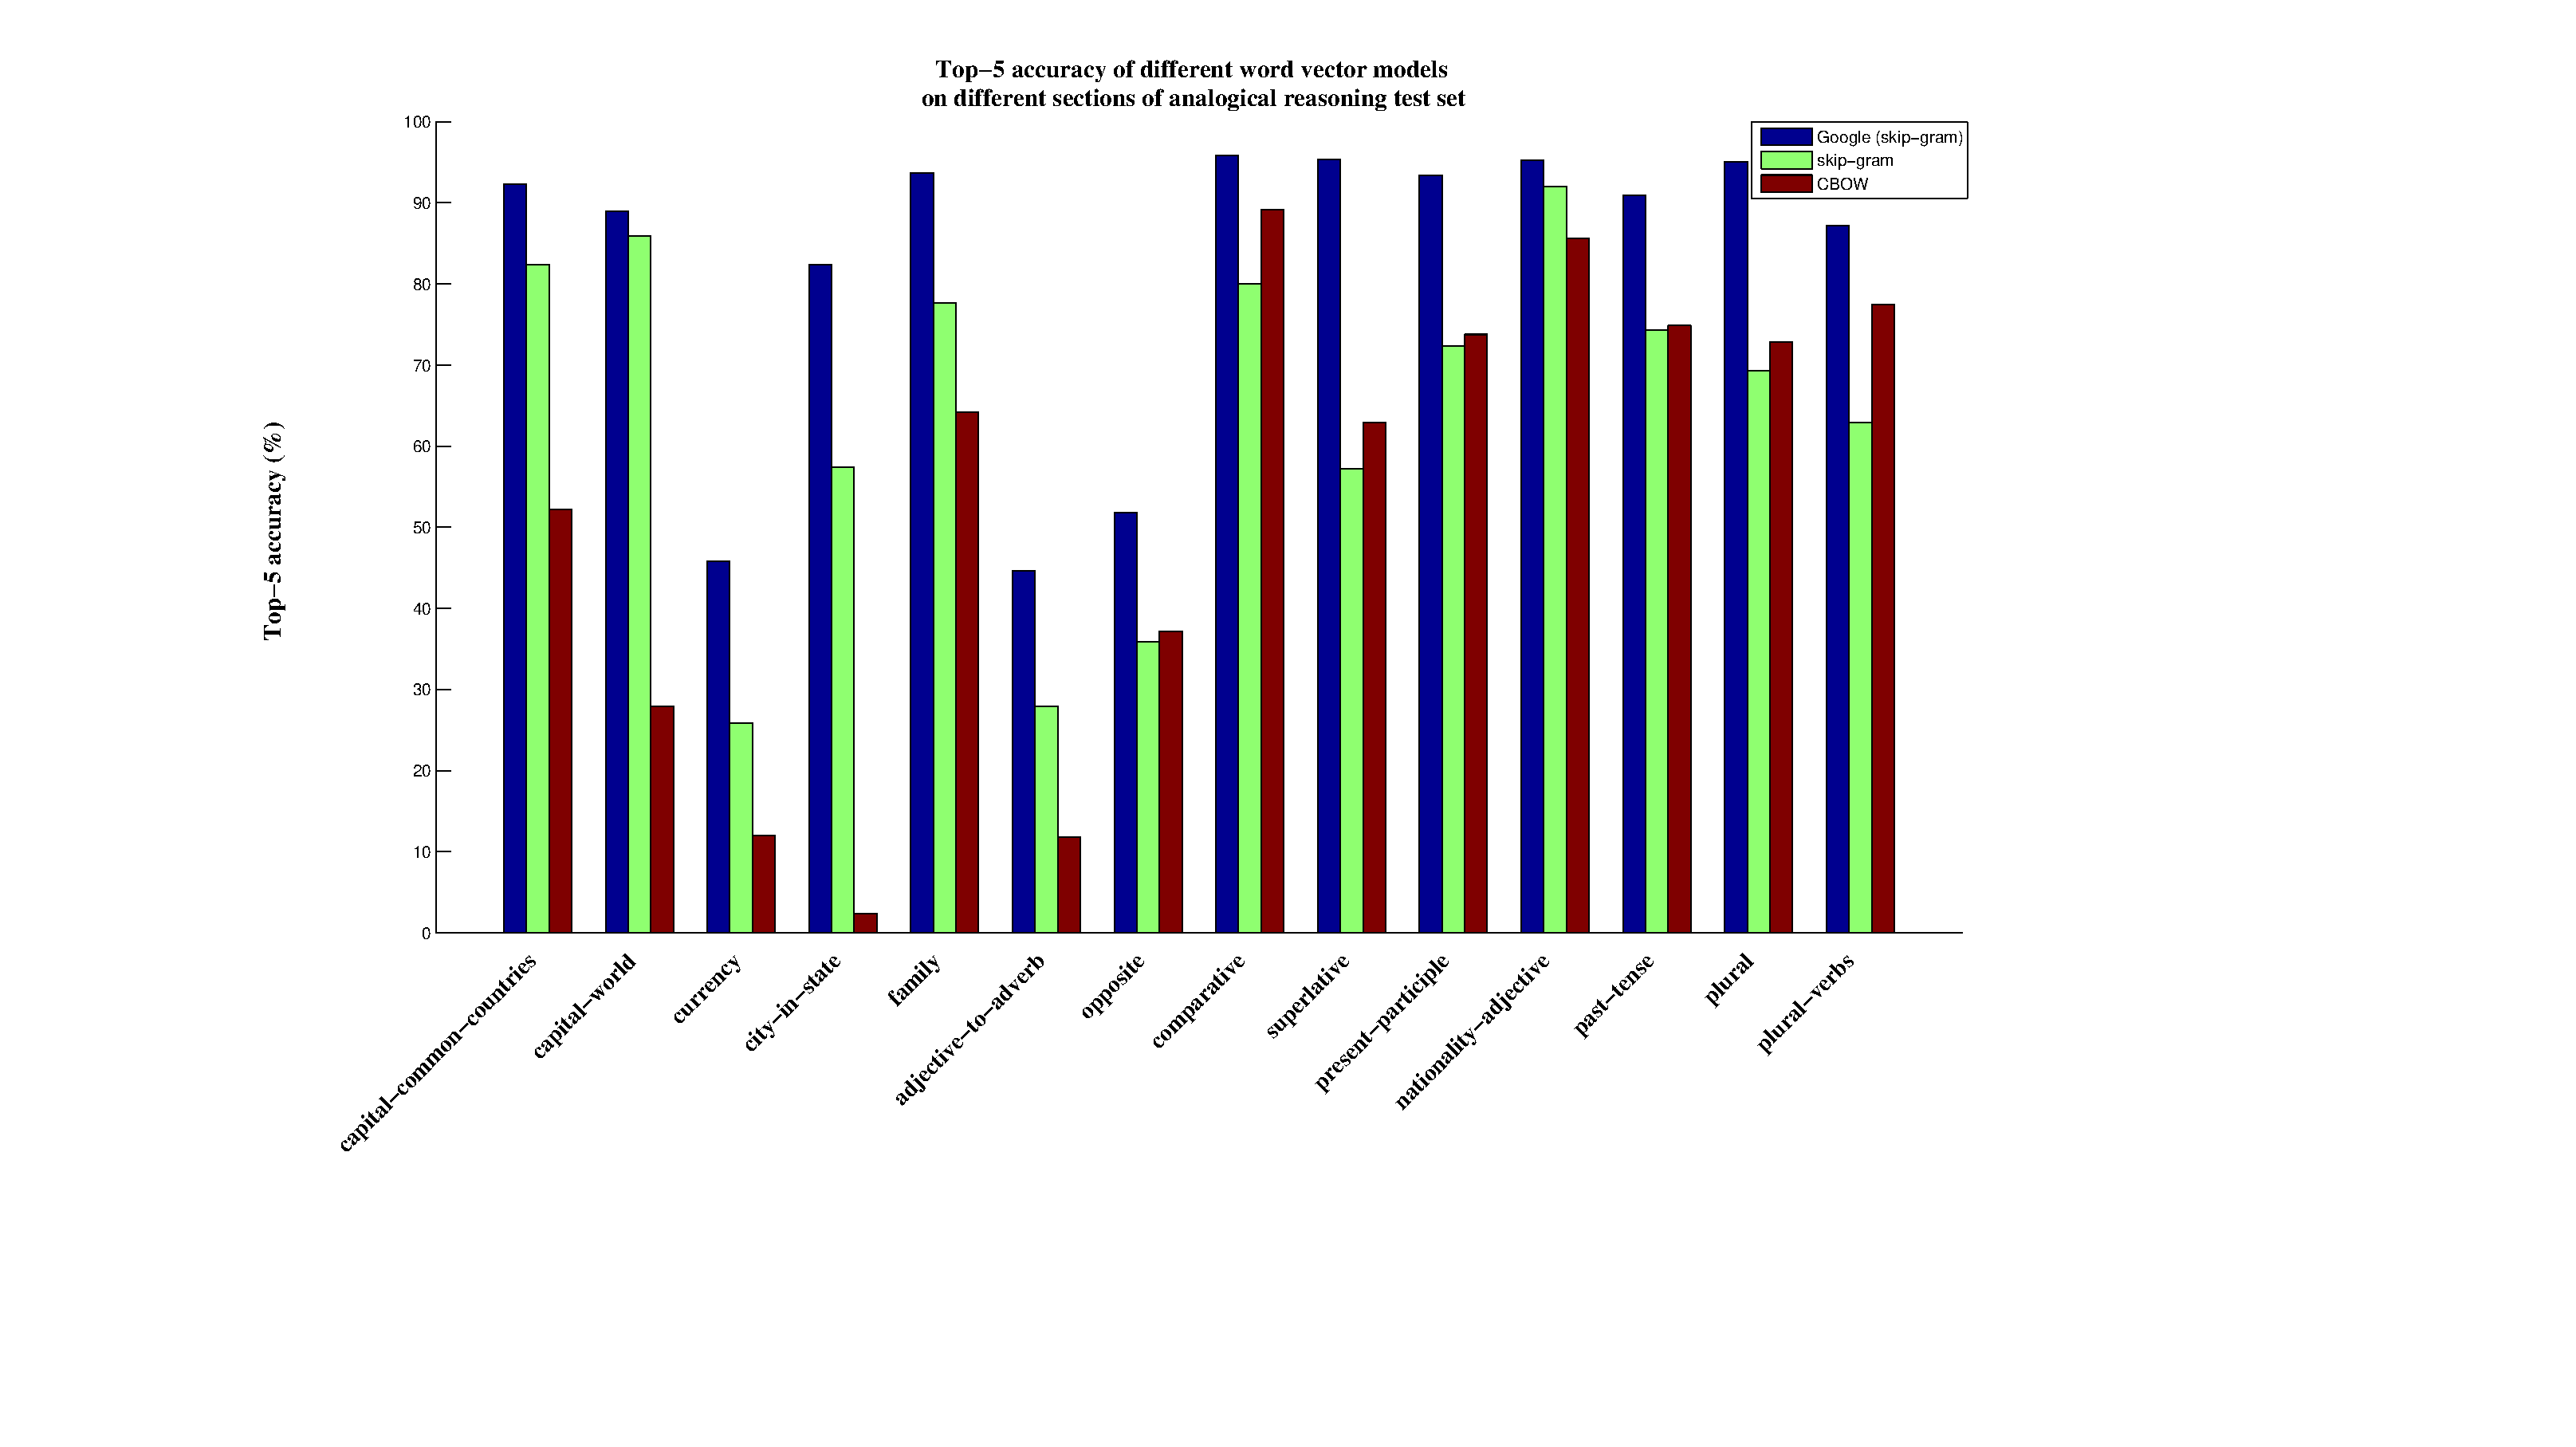
\includegraphics[width=\textwidth]{./images/analog_accuracy_per_question.eps}
\caption{Top-5 accuracy per analogy question type.}
\label{fig:accuracy_per_question}
\end{figure}


\subsubsection{Visualizing low dimensional approximations of embedding space}

\subsubsection{Finding analogical relations}
